\documentclass[../summary.tex]{subfiles}

\begin{document}
	
	\section{Climate}
		
		\subsection{Climate trends and causes}
			\subsubsection{Climate change over geological cycles}
				We know climate change is partly a natural phenomenon because of the research done with Antarctic ice. Figure \ref{fig:1-antarctic-ice-records} clearly shows a natural cycle in temperatures over the last 800,000 years. Other evidence pointing to this conclusion can be found in landscapes which have been altered by moving glacial ice.
				\begin{figure}[h]
					\centering
					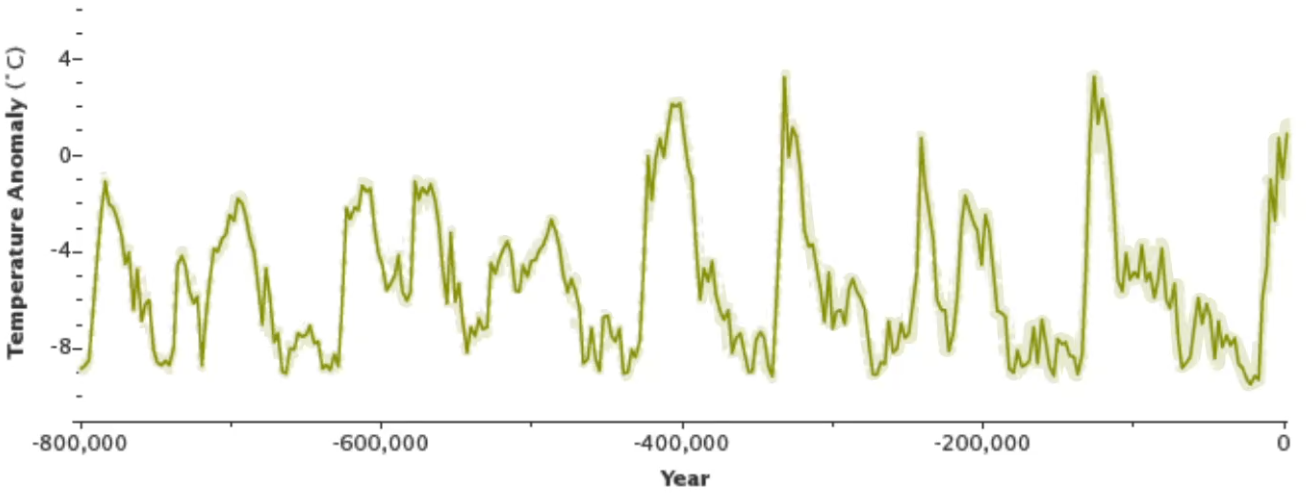
\includegraphics[width=0.7\linewidth]{../images/1-antarctic-ice-records.png}
					\caption{Antarctic ice records}
					\label{fig:1-antarctic-ice-records}
				\end{figure}
		\subsection{Climate targets and pathways}
		
		\subsection{Climate mitigation}
		
		\subsection{What can we expect for the future}
	
\end{document}